% ICIUS 2026 revision of submission UN006 (IEEEtran, conference option; no ICIUS template supplied).
% Every number in the text comes from generated/numbers.tex and every results table from
% generated/*.tex, both written by scripts/make_icius.py from the per-seed results.
\documentclass[conference]{IEEEtran}
\usepackage{amsmath,amssymb,amsthm}
\usepackage{graphicx}
\usepackage{booktabs}
\usepackage{cite}
\usepackage{algorithm}
\usepackage{algpseudocode}
\usepackage{url}
\newtheorem{lemma}{Lemma}
\newtheorem{proposition}{Proposition}
% generated by paper_icius/scripts/make_icius.py -- do not edit
\newcommand{\nAlt}{30}
\newcommand{\nArea}{400}
\newcommand{\nBudget}{113}
\newcommand{\nBw}{20}
\newcommand{\nChi}{0.70}
\newcommand{\nClo}{0.40}
\newcommand{\nCompHi}{11}
\newcommand{\nCompLo}{4}
\newcommand{\nDenseArea}{200}
\newcommand{\nDenseFusHi}{0.865}
\newcommand{\nDenseFusLo}{0.815}
\newcommand{\nDenseN}{50}
\newcommand{\nDenseNaive}{0.656}
\newcommand{\nDenseNofus}{0.740}
\newcommand{\nDenseS}{0.809}
\newcommand{\nDenseSigAbove}{B4}
\newcommand{\nDuration}{600}
\newcommand{\nEightArea}{100}
\newcommand{\nEightFastB}{0.62}
\newcommand{\nEightFastS}{0.60}
\newcommand{\nEightMaxDiff}{0.07}
\newcommand{\nEightN}{3}
\newcommand{\nEightSitlB}{0.60}
\newcommand{\nEightSitlS}{0.53}
\newcommand{\nEightWorlds}{3}
\newcommand{\nEoneDenseMappo}{0.779}
\newcommand{\nEoneDenseS}{0.809}
\newcommand{\nEoneNmax}{50}
\newcommand{\nEoneNmin}{3}
\newcommand{\nEoneTwoHundredSigN}{50}
\newcommand{\nEthreeGainHi}{29}
\newcommand{\nEthreeGainLo}{23}
\newcommand{\nEtwoSevB}{0.377}
\newcommand{\nEtwoSevBname}{B0}
\newcommand{\nEtwoSevS}{0.433}
\newcommand{\nEtwoUrbanB}{0.475}
\newcommand{\nEtwoUrbanBname}{B3}
\newcommand{\nEtwoUrbanS}{0.575}
\newcommand{\nFailRate}{0.01}
\newcommand{\nFlank}{15}
\newcommand{\nFlankAngle}{26.6}
\newcommand{\nFlankSlant}{12}
\newcommand{\nFoot}{12}
\newcommand{\nFreq}{2.4}
\newcommand{\nGant}{2}
\newcommand{\nGate}{5}
\newcommand{\nGth}{5}
\newcommand{\nLossAvgMax}{0.9}
\newcommand{\nLossWorst}{8.5}
\newcommand{\nLossWorstS}{3.2}
\newcommand{\nMissions}{13\,000}
\newcommand{\nNF}{7}
\newcommand{\nNineArea}{25}
\newcommand{\nNineAssocHi}{10}
\newcommand{\nNineAssocLo}{7}
\newcommand{\nNineBone}{0.63}
\newcommand{\nNineBzero}{0.67}
\newcommand{\nNineN}{3}
\newcommand{\nNineS}{0.71}
\newcommand{\nNoise}{-94}
\newcommand{\nNuav}{8}
\newcommand{\nPLzero}{40}
\newcommand{\nPlanPeriod}{1}
\newcommand{\nPsoC}{2.05}
\newcommand{\nPsoChi}{0.7298}
\newcommand{\nPtx}{20}
\newcommand{\nRunsOff}{21}
\newcommand{\nRunsOn}{1}
\newcommand{\nRurbanOne}{48}
\newcommand{\nRurbanZero}{91}
\newcommand{\nSeedMax}{29}
\newcommand{\nSeeds}{30}
\newcommand{\nStepsAll}{1\,317\,947}
\newcommand{\nStepsOff}{1\,868}
\newcommand{\nStepsOn}{1\,663}
\newcommand{\nStrictHi}{0.13}
\newcommand{\nStrictLo}{0.03}
\newcommand{\nTh}{116}
\newcommand{\nThList}{0,15,30,60,120,240,\infty}
\newcommand{\nThSevBest}{15}
\newcommand{\nThSevBestV}{0.501}
\newcommand{\nThSevGain}{20}
\newcommand{\nThSevInf}{0.419}
\newcommand{\nThSevLatBest}{41}
\newcommand{\nThSevLatInf}{74}
\newcommand{\nThUrbBest}{15}
\newcommand{\nThUrbBestV}{0.599}
\newcommand{\nThUrbGain}{15}
\newcommand{\nThUrbInf}{0.523}
\newcommand{\nThUrbLatBest}{16}
\newcommand{\nThUrbLatInf}{16}
\newcommand{\nUrbBestFus}{0.507}
\newcommand{\nUrbBestFusName}{B3}
\newcommand{\nUrbNodel}{0.523}
\newcommand{\nUrbNofus}{0.519}
\newcommand{\nUrbNofusNosa}{0.543}
\newcommand{\nUrbNonethree}{0.524}
\newcommand{\nUrbS}{0.575}
\newcommand{\nVeGflops}{8.7}
\newcommand{\nVeMap}{0.947}
\newcommand{\nVeMapB}{0.520}
\newcommand{\nVeParams}{3.14}
\newcommand{\nVeTrt}{1.73}
\newcommand{\nVictims}{25}
\newcommand{\nViolAll}{65}
\newcommand{\nViolFold}{37}
\newcommand{\nViolOff}{42}
\newcommand{\nViolOn}{1}
\newcommand{\nViolP}{10^{-4}}
\newcommand{\nViolRate}{4.9\times10^{-5}}
\newcommand{\nVmax}{5}
\newcommand{\nYnFlopRed}{31}
\newcommand{\nYnGflops}{6.0}
\newcommand{\nYnMap}{0.948}
\newcommand{\nYnMapB}{0.533}
\newcommand{\nYnParamRed}{19}
\newcommand{\nYnParams}{2.53}
\newcommand{\nYnTrt}{1.81}


\begin{document}
\title{Edge-AI Driven Elastic Mesh PSO for Low-Altitude UAV IoT Networks in Zero-Infrastructure Environments}

\author{\IEEEauthorblockN{Karthik KS}
\IEEEauthorblockA{CSE (AI\&ML), SRM IST\\Tiruchirappalli, India\\karthikzofficialmail@gmail.com}
\and
\IEEEauthorblockN{Nicholas Christo T}
\IEEEauthorblockA{CSE (AI\&ML), SRM IST\\Tiruchirappalli, India\\nicholastchristos@gmail.com}
\and
\IEEEauthorblockN{Balaji Ganesh Rajagopal}
\IEEEauthorblockA{School of Computing, SRM IST\\Tiruchirappalli, India\\balajiganesh.r@ist.srmtrichy.edu.in}}

\maketitle

\begin{abstract}
A low-altitude UAV swarm searching a disaster area without infrastructure must also carry each
victim report back to the responders over its own radio links. SENTINEL treats the swarm network as
an elastic mesh: it stretches and breaks while UAVs search, and is re-formed only when a confirmed
report must reach the responder. Elastic-Mesh PSO (EM-PSO) plans waypoints with a Signal-Spring that
penalises predicted link outage instead of distance; delivery is triggered by the information each UAV
has confirmed; and weak thermal detections are corroborated from a second viewpoint. A local
minimum-spanning-tree projection keeps the delivery path reliable for every feasible step. In about
\nMissions{} simulated missions with a \nFreq\,GHz outage channel model, \nEoneNmin--\nEoneNmax{} UAVs, six failure
settings and seven tuned baselines (\nSeeds{} seeds, paired tests), SENTINEL reports \nEthreeGainLo--\nEthreeGainHi\,\%
more victims within 60\,s than the best baseline in urban rubble, and PX4 software-in-the-loop runs
agree with the simulator. Keeping the mesh connected at all times lowers timely reporting.
\end{abstract}

\begin{IEEEkeywords}
UAV swarm, edge AI, particle swarm optimization, search and rescue, intermittent connectivity,
low-altitude IoT.
\end{IEEEkeywords}

\section{Introduction}
After an earthquake or a collapse, small multirotor UAVs with thermal cameras can cover rubble
quickly, and compact detectors make it possible to find people on board instead of streaming video to
a server \cite{hituav,yolo26}. A detection is useful, however, only once the responders receive it,
and without infrastructure the report travels over the UAVs' own short-range links, which buildings
block, fading weakens and failures cut. A swarm that stays connected delivers every report at once but
searches a small area; a swarm that explores freely finds more victims but leaves delivery to chance.
We call this the \emph{discovery--delivery trade-off} and measure it directly: the share of victims
whose report reaches the responder within 60\,s.

Our first version of SENTINEL addressed the problem with a quadratic spring that kept each UAV within
a fixed 50\,m of its nearest neighbour. Three things were wrong with that design. A fixed radius says
nothing about a link behind rubble; keeping the nearest neighbour close does not keep the network
connected (Lemma~\ref{lem:nn}); and a \nNineArea\,m test area is smaller than the radio range, so every method
stays connected there and the methods barely differ (Section~\ref{sec:sitl}). This revision
keeps the elastic-mesh idea but changes what it means. The mesh is free to stretch and break during
search and is re-formed for delivery only. The contributions are:
\begin{itemize}
\item \textbf{EM-PSO with an outage-based Signal-Spring}, which penalises the predicted outage of a
link under path loss, obstructions, shadowing and fading, and is active only while a report is being
delivered.
\item \textbf{Information-triggered delivery}: a UAV leaves the search when a victim it confirmed has
not reached the responder within a hold time $T_h$.
\item \textbf{Corroborative multi-view sensing}: a weak detection asks a neighbour for a lateral second
view, and views are fused so that an occluded angle cannot veto a clear one.
\item \textbf{A statistical evaluation} against seven tuned baselines with \nEoneNmin--\nEoneNmax{} UAVs, four
channel profiles and six failure settings, with confidence intervals and paired tests, plus a PX4/Gazebo
cross-check. Code, scenarios and results are released.
\end{itemize}

\section{Related Work}
Connectivity-maintenance controllers keep the communication graph connected at every instant, by
following the gradient of its algebraic connectivity $\lambda_2$ \cite{zavlanos2008,sabattini2013} or
with edge potentials that grow without bound near the range limit \cite{ji2007}; local topology
control such as the local minimum spanning tree (LMST) reduces the links that must be kept
\cite{li2003lmst}. These methods tie the whole team to the network and assume a disk radio model.
Intermittent-connectivity planning lets robots disconnect and meet on a schedule \cite{kantaros2017},
data ferrying moves data between known sources and a sink \cite{cui2023ferry}, and age-of-information
work optimises the freshness of collected data \cite{kaul2012aoi,bafarassat2026aoi}; all of them know
the sources or the meetings in advance, whereas the victims are found by the search itself.
Distributed PSO and Bayesian multi-UAV search \cite{clerc2002,yang2024dapso,niu2026eventbayes,zhu2026mountain}
assume communication is available when needed, and multi-agent reinforcement learning, with MAPPO as a
strong general method \cite{yu2022mappo}, has been applied to communication-aware UAV coordination
\cite{shi2025symmetry}. SENTINEL combines online-discovered sources, a reporting deadline, an
obstruction- and fading-aware channel and failure-aware evaluation (Table~\ref{tab:related}).
\begin{table}[t]\centering\caption{Closest approaches (\checkmark: addressed; $\circ$: partly; --: not addressed).}\label{tab:related}
\footnotesize\setlength{\tabcolsep}{2.2pt}
\begin{tabular}{@{}lccccc@{}}\toprule
Approach & \shortstack{online\\sources} & deadline & \shortstack{obstr./\\fading} & failures & \shortstack{free\\search}\\\midrule
$\lambda_2$ control \cite{zavlanos2008,sabattini2013} & -- & -- & -- & $\circ$ & -- \\
Edge potentials \cite{ji2007} & -- & -- & -- & -- & -- \\
Intermittent conn.\ \cite{kantaros2017} & -- & $\circ$ & -- & -- & \checkmark \\
Ferrying / AoI \cite{cui2023ferry,bafarassat2026aoi} & -- & \checkmark & $\circ$ & -- & \checkmark \\
PSO / Bayesian search \cite{yang2024dapso,niu2026eventbayes} & \checkmark & -- & -- & -- & \checkmark \\
MARL \cite{yu2022mappo,shi2025symmetry} & $\circ$ & $\circ$ & $\circ$ & $\circ$ & \checkmark \\
Our first version & \checkmark & -- & -- & $\circ$ & $\circ$ \\
\textbf{SENTINEL} & \checkmark & \checkmark & \checkmark & \checkmark & \checkmark \\\bottomrule
\end{tabular}\end{table}

\section{System Model}\label{sec:model}
$N$ UAVs fly at altitude $h$ over an area with tall buildings (no-fly zones that also block radio
links) and low rubble that hides victims. A responder radio (node 0) at the launch point is the only
sink for reports. Every slot $\Delta t$ each UAV broadcasts a status message with its position, its
target ledger and acknowledgements.

\emph{Channel.} The SINR of the broadcast from $i$ at $j$ is
\begin{equation}
\gamma_{ij}=\frac{P_t G^2\,10^{-(\mathrm{PL}(d_{ij})+n_{ij}L_o+X_{ij})/10}\,|h_{ij}|^2}{\sigma^2+\sum_{k\in\mathcal{I}_j}\bar P_{kj}},\label{eq:sinr}
\end{equation}
with log-distance path loss $\mathrm{PL}(d)=\mathrm{PL}(d_0)+10\eta\log_{10}(d/d_0)$, $n_{ij}$
obstacles crossing the link with loss $L_o$ each, shadowing $X_{ij}\sim\mathcal{N}(0,\sigma_X^2)$
correlated over displacement \cite{gudmundson1991}, unit-mean Rician fading $|h_{ij}|^2$ (Rayleigh
once obstructed) and colliding transmitters $\mathcal{I}_j$. A packet is decoded iff
$\gamma_{ij}\ge\gamma_{\mathrm{th}}$. The outage probability averaged over fading and shadowing is
\begin{equation}
P_{\mathrm{out}}(d,n)=\mathbb{E}_X\big[F_{|h|^2}\big(\gamma_{\mathrm{th}}/(\bar\gamma(d,n)\,10^{X/10})\big)\big],\label{eq:pout}
\end{equation}
and the \emph{reliable range} is $R_\varepsilon(n)=\max\{d:P_{\mathrm{out}}(d,n)\le\varepsilon\}$.
The link budget uses $f=\nFreq$\,GHz, $P_t=\nPtx$\,dBm, $G=\nGant$\,dBi per side, $B=\nBw$\,MHz,
noise figure \nNF\,dB (noise floor \nNoise\,dBm) and $\gamma_{\mathrm{th}}=\nGth$\,dB, which allows
\nBudget\,dB of path loss before fading margins ($\mathrm{PL}(1\,\mathrm{m})=\nPLzero$\,dB). Profile
parameters follow the ranges reported for low-altitude and street-level links
\cite{tr36777,itup1411}. Table~\ref{tab:channel} gives the resulting ranges: in urban rubble
$R_{0.05}=\nRurbanZero$\,m with a clear line of sight and \nRurbanOne\,m behind one obstruction. The
50\,m radius of our first version therefore matches a link through one layer of rubble, and a second
obstruction or a harsher profile shrinks it further.
% generated by paper_icius/scripts/make_icius.py -- do not edit
\begin{table}[t]\centering\caption{Channel profiles and reliable ranges $R_{0.05}(n)$ for $n$ obstructions ($\sigma_X$, $L_o$ in dB).}\label{tab:channel}
\footnotesize\setlength{\tabcolsep}{3.5pt}\begin{tabular}{lcccccc}\toprule
Profile & $\eta$ & $\sigma_X$ & $K$ & $L_o$ & $R(0)$ [m] & $R(1)$ [m]\\\midrule
open & 2 & 2 & 10\,dB & 6 & 2434 & 684 \\
suburban & 2.5 & 4 & 6\,dB & 10 & 339 & 95 \\
urban rubble & 3 & 6 & 3\,dB & 6 & 91 & 48 \\
severe & 3.5 & 8 & Rayleigh & 8 & 35 & 21 \\
\bottomrule\end{tabular}\end{table}


\emph{Information and failures.} Each UAV keeps a ledger of world-frame victim entries; detections
within the association gate are merged, and an entry is \emph{confirmed} when its fused confidence
$c_e\ge c_{\mathrm{hi}}$ and \emph{tentative} when $c_{\mathrm{lo}}\le c_e<c_{\mathrm{hi}}$. Ledgers
spread by gossip with acknowledgements; an entry is \emph{secured} once the responder holds it and
\emph{lost} if every UAV holding it fails first. UAVs fail by crashing (with their ledger), by radio
loss or by a gradual transmit-power brownout, singly, simultaneously, in cascades or as a Poisson
process.

\emph{Objective.} Let $\tau_k$ be the time victim $k$ is first confirmed and $T_k$ the time, from
mission start, at which its report reaches the responder ($T_k=\infty$ if never). The team maximises
\begin{equation}
J=\frac{1}{|\mathcal{V}|}\sum_{k\in\mathcal{V}}e^{-T_k/\theta}\label{eq:J}
\end{equation}
under decentralised information. Staying connected makes delivery immediate but limits discovery;
free search does the opposite.

\section{SENTINEL}\label{sec:method}
\emph{Mode switching.} Let $\mathcal{E}_i(t)$ be the confirmed, unsecured entries UAV $i$ is
responsible for (it created them, or they are older than $3T_h$). UAV $i$ switches from
\textsc{Explore} to \textsc{Deliver} when
\begin{equation}
\max_{e\in\mathcal{E}_i(t)}(t-\tau_e)\ge T_h\label{eq:trigger}
\end{equation}
and back when $\mathcal{E}_i(t)=\emptyset$. $T_h=0$ delivers every confirmation at once;
$T_h\to\infty$ never interrupts the search. Connection to the responder is known locally from a
time stamp that the responder issues and every UAV relays.

\emph{EM-PSO.} Each planning period the UAV picks a waypoint in its reachable disk $\mathcal{D}_i$ by
maximising
\begin{multline}
F_i(x)=w_c\hat G_i(x)+w_d\!\!\sum_{e\in\mathcal{T}_i}\!c_e e^{-\frac{\|x-x_e\|^2}{2s^2}}\\
+\frac{w_g(\|x_i-g_i\|-\|x-g_i\|)-w_t\|x-x_i\|}{vT_p}-S_i(x),\label{eq:fitness}
\end{multline}
where $\hat G_i$ is the expected number of new detections of a look at $x$ on the UAV's search map,
$\mathcal{T}_i$ the tentative entries, $g_i$ a frontier goal and $w_t$ a small travel cost. The
Signal-Spring acts only while the UAV is tethered (delivering and connected, or relaying a delivery):
\begin{equation}
S_i(x)=\lambda_i\!\sum_{j\in\mathcal{S}_i}\!\left(\frac{[P_{\mathrm{out}}(\|x-x_j\|,n(x,x_j))-\varepsilon_i]_+}{\varepsilon_i}\right)^{\!2},\label{eq:spring}
\end{equation}
with $\lambda_i=\lambda_0(1+\beta U_i)$, $\varepsilon_i=\varepsilon/(1+\beta U_i)$ and $U_i$ the
number of entries only $i$ holds. It penalises predicted outage rather than distance, so it accounts
for obstructions, and it tightens with the unique information a UAV carries. A
constriction-coefficient PSO ($\chi=\nPsoChi$, $c_1=c_2=\nPsoC$) \cite{clerc2002} maximises $F_i$.

\emph{Link preservation.} $\mathcal{S}_i$ contains the neighbours adjacent to $i$ in the minimum
spanning tree of the reliable graph among the neighbours $i$ has heard \cite{li2003lmst}. If all UAVs use the same positions and have heard all
their reliable neighbours, the mutually selected edges contain the global minimum spanning forest and
so preserve the connected components.
\begin{lemma}\label{lem:nn}
Nearest-neighbour distance constraints do not imply connectivity.
\end{lemma}
\begin{proof}
UAVs at $(0,0),(10,0),(200,0),(210,0)$ with $R=50$\,m each have a neighbour at 10\,m, yet no edge joins
the two pairs.
\end{proof}
While tethered, UAV $i$ scales its step $u_i$ to the largest $\alpha\in[0,1]$ such that
$x_i'=x_i+\alpha u_i$ satisfies, for all $j\in\mathcal{S}_i$,
\begin{equation}
\|x_i'-m_{ij}\|\le\tfrac12 r_{ij}(x_i')-\tfrac12 v\,a_{ij},\quad r_{ij}=R_\varepsilon\big(n^{\delta_{ij}}(x_i',\hat x_j)\big),\label{eq:proj}
\end{equation}
where $\hat x_j$ is $j$'s last reported position of age $a_{ij}$, $m_{ij}=(x_i+\hat x_j)/2$,
$\delta_{ij}=v(\Delta t+a_{ij})$ and $n^\delta$ counts obstacles inflated by $\delta$.
\begin{proposition}\label{prop:link}
If $j\in\mathcal{S}_i$, $i\in\mathcal{S}_j$, both UAVs are tethered, speeds are bounded by $v$,
positions are exchanged with staleness at most $a$, and both steps satisfy \eqref{eq:proj}, then link
$(i,j)$ is $\varepsilon$-reliable at $t+\Delta t$.
\end{proposition}
\begin{proof}[Proof sketch]
Each midpoint estimate is within $va/2$ of the true midpoint, so the triangle inequality and
\eqref{eq:proj} give $\|x_i'-x_j'\|\le\frac12(r_{ij}+r_{ji})$. The new segment lies within
$\delta_{ij}$ of $[x_i',\hat x_j]$, so the inflated count bounds the true one, and since $R_\varepsilon$
is non-increasing in $n$, $\|x_i'-x_j'\|\le R_\varepsilon(n(x_i',x_j'))$.
\end{proof}
The guarantee holds for feasible steps; if \eqref{eq:proj} is infeasible the UAV hovers, and we
measure the resulting violations (Section~\ref{sec:safety}).

\emph{Corroborative sensing.} A tentative entry ($c_{\mathrm{lo}}\le c_e<c_{\mathrm{hi}}$, with
$c_{\mathrm{lo}}=\nClo$, $c_{\mathrm{hi}}=\nChi$) asks the nearest neighbour for a view from
$\pm\nFlank$\,m perpendicular to the observer--target line, admitted only if the flank point keeps
that neighbour's preserved links feasible. At $h=\nAlt$\,m the flank views the victim
\nFlankAngle$^\circ$ off nadir, enough to look past the edge of a covering slab, while the slant range
grows by only \nFlankSlant\,\%, so the detector's range penalty stays small. The ledger keeps the best confidence $c_{e,v}$ per viewing
sector $v$. Naive-Bayes fusion treats a weak view from a blocked side as evidence of absence; with many
UAVs such views outvote a clear one. SENTINEL fuses corroboratively,
\begin{equation}
\mathrm{logit}\,c_e=\max_v\mathrm{logit}\,c_{e,v}+\sum_{v\ne v^\star}[\mathrm{logit}\,c_{e,v}]_+,\label{eq:fusion}
\end{equation}
where $v^\star$ is the best view; other views can only add support.

\emph{Complexity.} A planning step evaluates $P$ particles for $I$ iterations, each costing $O(k)$
outage look-ups for $k=|\mathcal{S}_i|$ preserved neighbours, and the local spanning tree costs
$O(k_h^2\log k_h)$ for the $k_h$ neighbours heard; no term grows with $N$ directly, unlike the
swarm-wide eigenvector needed by $\lambda_2$ control. Because the hinge in \eqref{eq:spring} is
squared, $S_i$ is continuously differentiable and adds no kink to the fitness.

\begin{algorithm}[t]\small\caption{SENTINEL agent $i$ (every slot $\Delta t$)}\label{alg:agent}
\begin{algorithmic}[1]
\State record look; add geolocated detections to the ledger
\State broadcast status $(x_i,\text{ledger},\text{acks},\text{stamp},t_{\mathrm{tether}})$; merge received ones
\If{planning slot}
  \State update mode with \eqref{eq:trigger}; request flanks for own tentative entries
  \If{\textsc{Deliver} and not connected} \State waypoint $\gets x_0$
  \Else \State waypoint $\gets\arg\max_{x\in\mathcal{D}_i}F_i(x)$ by PSO \Comment{$S_i{\equiv}0$ unless tethered}
  \EndIf
\EndIf
\State $u_i\gets$ step toward waypoint; \textbf{if} tethered, scale by $\alpha^\star$ from \eqref{eq:proj}
\State $x_i\gets x_i+u_i$
\end{algorithmic}
\end{algorithm}

\section{Implementation}
The algorithms form one ROS-independent Python library, executed both by a fast multi-agent simulator
and by ROS~2 Humble nodes that fly PX4 x500 quadrotors in Gazebo Harmonic through Micro XRCE-DDS
(Fig.~\ref{fig:graph}). Each UAV runs a flight commander, a thermal-vision node (YOLO26n with
geolocation), the SENTINEL agent and a camera bridge; all inter-UAV traffic passes through a radio
emulator that drops packets by sampled SINR. UAVs fly at $h=\nAlt$\,m and $v=\nVmax$\,m/s with a
\nFoot\,m camera footprint; $T_h=\nTh$\,s and the other free parameters were tuned
(Section~\ref{sec:eval}); Table~\ref{tab:params} lists the defaults. Worlds are generated from the
same seeds as the fast simulator, with heated Rescue Randy mannequins lying in the open or partly
under concrete slabs and warm debris that causes false alarms (Fig.~\ref{fig:scene}).
% generated by paper_icius/scripts/make_icius.py -- do not edit
\begin{table}[t]\centering\caption{Default parameters (from the code and the tuned configuration).}\label{tab:params}
\footnotesize\setlength{\tabcolsep}{3pt}\begin{tabular}{@{}lp{0.76\columnwidth}@{}}\toprule
Kinematics & $\Delta t=0.5$\,s, $v=5$\,m/s, $h=30$\,m, footprint 12\,m\\
Planning & every 1\,s, horizon $T_p=4$\,s, PSO $P=24$, $I=12$\\
Tuned & $T_h=116$\,s, $\lambda_0=1.20$, $\beta=1.09$, $w_g=0.066$\\
Spring & $\varepsilon=0.05$, $w_c=1$, $w_d=1$, $w_t=0.05$\\
Sensing & $c_{\mathrm{lo}}=0.40$, $c_{\mathrm{hi}}=0.70$, flank $\pm15$\,m, gate 5\,m, 8 sectors\\
Detector & $c_{\max}=0.92$, $\gamma=1.5$, $r_{\mathrm{ref}}=35$\,m, $\sigma_c=0.08$, false alarms 0.02/look\\
\bottomrule\end{tabular}\end{table}

\begin{figure}[t]\centering
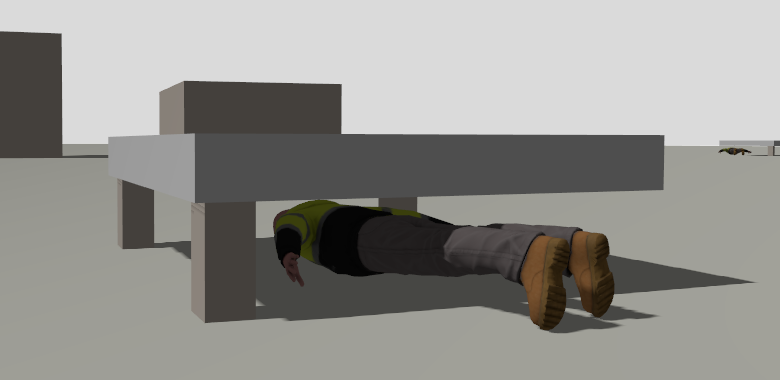
\includegraphics[width=0.85\columnwidth]{figures/S2_victims_occlusion.png}\\[2pt]
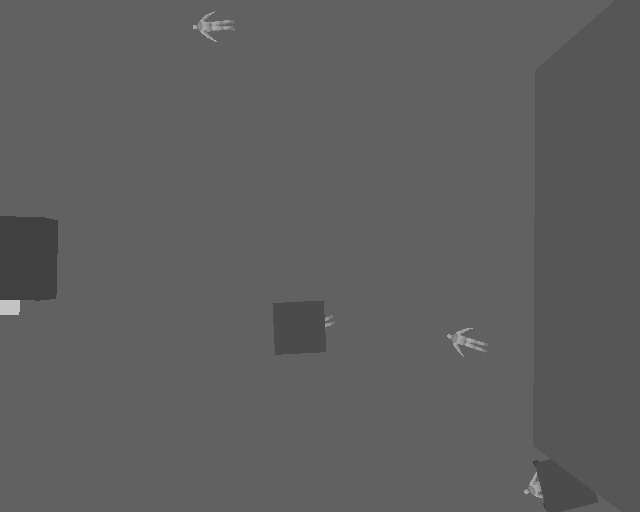
\includegraphics[width=0.5\columnwidth]{figures/S4_thermal_frame.png}
\caption{Gazebo scene. Top: a victim partly under a slab (torso hidden from above). Bottom:
white-hot thermal frame from a UAV at \nAlt\,m with victims in the open, under slabs and warm debris.}
\label{fig:scene}
\end{figure}
\begin{figure}[t]\centering
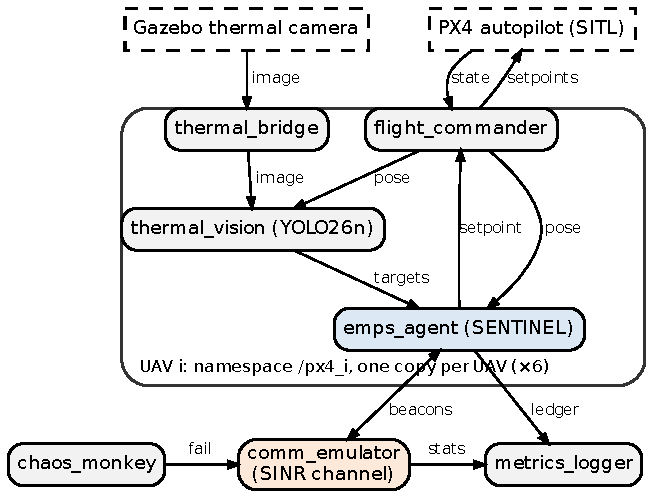
\includegraphics[width=\columnwidth]{figures/ros_graph.pdf}
\caption{ROS~2 node graph, transcribed from the running six-UAV system; one copy of the four UAV
nodes runs per UAV, and UAVs exchange data only through the radio emulator.}\label{fig:graph}
\end{figure}

\section{Evaluation}\label{sec:eval}
\emph{Setup.} Each run generates a new disaster area from its seed (no-fly buildings, rubble, warm
debris, \nVictims{} victims of which one is buried) and lasts \nDuration\,s. Unless stated, the area
is \nArea$\times$\nArea\,m, $N=\nNuav$, the channel is urban rubble and UAVs fail as a Poisson process
at \nFailRate\,s$^{-1}$ per swarm. The detector
in the loop is a parameterised model of confidence versus range and view-dependent occlusion with
false alarms from warm debris. The metric is the share of all victims reported to the responder
within 60\,s of first confirmation. It replaces the network-retention and discovery rates of our
first version, which were coarse for ten victims and one run, with a per-victim measure that counts
only reports that actually arrive. Baselines: B0 constriction PSO; B1 our first version (50\,m
nearest-neighbour spring); B2 PSO with an outage penalty on all neighbours; B3 $\lambda_2$-gradient
control \cite{sabattini2013} with the exact $\lambda_2$ (an oracle); B4 edge potentials with hysteresis
\cite{ji2007}; B5 MAPPO \cite{yu2022mappo}; B6 sweep search. Every method was tuned with the same
Optuna budget on $J$ using seeds that are never used for evaluation (MAPPO was trained to a plateau on
separate seeds). Each setting uses seeds 0--\nSeedMax{} with common random numbers; tables give the mean and
the half-width of the 95\,\% bootstrap confidence interval, and $^*$ marks a paired Wilcoxon test
against SENTINEL, Holm-corrected. The baselines keep the best single view per victim and request no
second views, as in their designs; Table~\ref{tab:attr} also gives them SENTINEL's fusion rule.

\emph{Channel and failures.} SENTINEL reports the most victims in every channel profile
(Table~\ref{tab:e2}), significantly more than all baselines except in the severe profile, where it
leads (\nEtwoSevS{} vs.\ \nEtwoSevB{}, \nEtwoSevBname) without significance. Under all six failure
settings in urban rubble it reports \nEthreeGainLo--\nEthreeGainHi\,\% more victims than the best
baseline (Table~\ref{tab:e3}). Losing a confirmed victim to failures is rare for every method
because ledgers spread by gossip: at most \nLossAvgMax\,\% averaged over the failure settings, and
\nLossWorst\,\% in the worst cell (twice the Poisson rate, severe channel; SENTINEL \nLossWorstS\,\%),
so we claim no advantage in information loss.
% generated by paper_icius/scripts/make_icius.py -- do not edit
\begin{table}[t]\centering\caption{Victims reported within 60\,s per channel profile (400\,m, $N=8$, Poisson failures). Mean $\pm$ half-width of the 95\,\% bootstrap CI over 30 seeds; best in bold; $^*$: differs from SENTINEL (paired Wilcoxon, Holm-corrected, $p<0.05$).}\label{tab:e2}
\footnotesize\setlength{\tabcolsep}{2pt}\begin{tabular}{lcccc}\toprule
Method & open & suburban & urban & severe\\\midrule
SENTINEL & \textbf{0.58$\pm$0.04} & \textbf{0.56$\pm$0.05} & \textbf{0.57$\pm$0.05} & \textbf{0.43$\pm$0.05} \\
B0 PSO & 0.47$\pm$0.05$^*$ & 0.46$\pm$0.05$^*$ & 0.45$\pm$0.04$^*$ & 0.38$\pm$0.05 \\
B1 v1 spring & 0.46$\pm$0.05$^*$ & 0.43$\pm$0.05$^*$ & 0.41$\pm$0.05$^*$ & 0.37$\pm$0.05 \\
B2 comm-PSO & 0.47$\pm$0.05$^*$ & 0.37$\pm$0.04$^*$ & 0.47$\pm$0.04$^*$ & 0.34$\pm$0.05$^*$ \\
B3 $\lambda_2$-grad. & 0.48$\pm$0.05$^*$ & 0.45$\pm$0.05$^*$ & 0.47$\pm$0.04$^*$ & 0.35$\pm$0.06 \\
B4 potential & 0.50$\pm$0.05$^*$ & 0.10$\pm$0.03$^*$ & 0.13$\pm$0.04$^*$ & 0.30$\pm$0.06$^*$ \\
B5 MAPPO & 0.41$\pm$0.05$^*$ & 0.42$\pm$0.04$^*$ & 0.40$\pm$0.05$^*$ & 0.33$\pm$0.05$^*$ \\
B6 sweep & 0.42$\pm$0.05$^*$ & 0.42$\pm$0.05$^*$ & 0.42$\pm$0.05$^*$ & 0.37$\pm$0.05 \\
\bottomrule\end{tabular}\end{table}

% generated by paper_icius/scripts/make_icius.py -- do not edit
\begin{table*}[t]\centering\caption{Victims reported within 60\,s under six failure settings (urban rubble, 400\,m, $N=8$). Mean $\pm$ half-width of the 95\,\% bootstrap CI over 30 seeds; best in bold; $^*$: differs from SENTINEL (paired Wilcoxon, Holm-corrected, $p<0.05$).}\label{tab:e3}
\footnotesize\setlength{\tabcolsep}{4pt}\begin{tabular}{lcccccc}\toprule
Method & none & single crash & 30\,\% simult. & cascading & Poisson$\times$2 & brownout\\\midrule
SENTINEL & \textbf{0.69$\pm$0.04} & \textbf{0.69$\pm$0.04} & \textbf{0.67$\pm$0.04} & \textbf{0.64$\pm$0.04} & \textbf{0.46$\pm$0.05} & \textbf{0.69$\pm$0.04} \\
B0 PSO & 0.54$\pm$0.04$^*$ & 0.52$\pm$0.04$^*$ & 0.51$\pm$0.04$^*$ & 0.51$\pm$0.04$^*$ & 0.34$\pm$0.06$^*$ & 0.54$\pm$0.04$^*$ \\
B1 v1 spring & 0.50$\pm$0.05$^*$ & 0.50$\pm$0.05$^*$ & 0.50$\pm$0.05$^*$ & 0.49$\pm$0.05$^*$ & 0.36$\pm$0.05$^*$ & 0.51$\pm$0.05$^*$ \\
B2 comm-PSO & 0.56$\pm$0.03$^*$ & 0.55$\pm$0.03$^*$ & 0.52$\pm$0.03$^*$ & 0.52$\pm$0.04$^*$ & 0.34$\pm$0.03$^*$ & 0.55$\pm$0.04$^*$ \\
B3 $\lambda_2$-grad. & 0.53$\pm$0.03$^*$ & 0.52$\pm$0.04$^*$ & 0.51$\pm$0.04$^*$ & 0.49$\pm$0.03$^*$ & 0.34$\pm$0.05$^*$ & 0.53$\pm$0.03$^*$ \\
B4 potential & 0.19$\pm$0.04$^*$ & 0.16$\pm$0.03$^*$ & 0.14$\pm$0.04$^*$ & 0.16$\pm$0.04$^*$ & 0.09$\pm$0.03$^*$ & 0.18$\pm$0.04$^*$ \\
B5 MAPPO & 0.50$\pm$0.04$^*$ & 0.47$\pm$0.04$^*$ & 0.45$\pm$0.04$^*$ & 0.46$\pm$0.04$^*$ & 0.33$\pm$0.05$^*$ & 0.49$\pm$0.04$^*$ \\
B6 sweep & 0.52$\pm$0.04$^*$ & 0.51$\pm$0.04$^*$ & 0.49$\pm$0.04$^*$ & 0.49$\pm$0.04$^*$ & 0.35$\pm$0.05$^*$ & 0.52$\pm$0.04$^*$ \\
\bottomrule\end{tabular}\end{table*}


\emph{Swarm size.} On the \nArea\,m area SENTINEL is significantly better than every baseline from
\nEoneNmin{} to \nEoneNmax{} UAVs (Table~\ref{tab:e1}). On a \nDenseArea\,m area, where contacts are frequent,
it has the highest mean at every size but is significantly better than all baselines only for
$N=\nEoneTwoHundredSigN$ (\nEoneDenseS{} vs.\ \nEoneDenseMappo{} for MAPPO). Planning takes
\nCompLo--\nCompHi\,ms per agent, well below the \nPlanPeriod\,s planning period.
% generated by paper_icius/scripts/make_icius.py -- do not edit
\begin{table}[t]\centering\caption{Victims reported within 60\,s vs.\ swarm size (400\,m, urban rubble, Poisson failures). Mean $\pm$ half-width of the 95\,\% bootstrap CI over 30 seeds; best in bold; $^*$: differs from SENTINEL (paired Wilcoxon, Holm-corrected, $p<0.05$).}\label{tab:e1}
\scriptsize\setlength{\tabcolsep}{1.6pt}\begin{tabular}{lccccc}\toprule
Method & $N=3$ & $N=5$ & $N=10$ & $N=20$ & $N=50$\\\midrule
SENTINEL & \textbf{0.20$\pm$0.04} & \textbf{0.39$\pm$0.06} & \textbf{0.67$\pm$0.04} & \textbf{0.75$\pm$0.03} & \textbf{0.79$\pm$0.03} \\
B0 PSO & 0.15$\pm$0.03$^*$ & 0.29$\pm$0.05$^*$ & 0.53$\pm$0.04$^*$ & 0.62$\pm$0.03$^*$ & 0.66$\pm$0.04$^*$ \\
B1 v1 spring & 0.11$\pm$0.03$^*$ & 0.23$\pm$0.05$^*$ & 0.50$\pm$0.05$^*$ & 0.65$\pm$0.03$^*$ & 0.71$\pm$0.04$^*$ \\
B2 comm-PSO & 0.15$\pm$0.04$^*$ & 0.31$\pm$0.05$^*$ & 0.53$\pm$0.04$^*$ & 0.64$\pm$0.04$^*$ & 0.69$\pm$0.03$^*$ \\
B3 $\lambda_2$-grad. & 0.14$\pm$0.04$^*$ & 0.27$\pm$0.05$^*$ & 0.53$\pm$0.04$^*$ & 0.64$\pm$0.04$^*$ & 0.67$\pm$0.03$^*$ \\
B4 potential & 0.02$\pm$0.01$^*$ & 0.03$\pm$0.02$^*$ & 0.24$\pm$0.05$^*$ & 0.49$\pm$0.05$^*$ & 0.71$\pm$0.04$^*$ \\
B5 MAPPO & 0.15$\pm$0.04$^*$ & 0.27$\pm$0.04$^*$ & 0.50$\pm$0.05$^*$ & 0.63$\pm$0.03$^*$ & 0.73$\pm$0.03$^*$ \\
B6 sweep & 0.15$\pm$0.04$^*$ & 0.27$\pm$0.05$^*$ & 0.44$\pm$0.04$^*$ & 0.49$\pm$0.04$^*$ & 0.62$\pm$0.03$^*$ \\
\bottomrule\end{tabular}\end{table}


\emph{What produces the gains.} Table~\ref{tab:attr} removes components on the same seeds. Removing
fusion (\nUrbNofus) or delivery (\nUrbNodel) lowers the urban share significantly from \nUrbS; keeping
the mesh connected at all times collapses it to \nStrictLo--\nStrictHi{} across regimes. Given
SENTINEL's fusion rule, the best urban baseline rises to \nUrbBestFus{} (\nUrbBestFusName) and stays
significantly below SENTINEL, as do all seven. With fusion, flank and delivery all removed SENTINEL still
reports \nUrbNonethree, above every baseline with fusion; the remaining differences from the baselines
are tuned exploration aids and responder re-attachment, which we do not claim as contributions. In
a dense \nDenseN-UAV swarm the picture changes: fusion is decisive for SENTINEL (\nDenseS{} vs.\
\nDenseNofus{} without it and \nDenseNaive{} with naive-Bayes fusion), but baselines given the same
rule reach \nDenseFusLo--\nDenseFusHi, and \nDenseSigAbove{} exceeds SENTINEL significantly. The delivery
trigger helps with eight UAVs (Fig.~\ref{fig:thold}): $T_h=\nThUrbBest$\,s
raises the share over never delivering from \nThUrbInf{} to \nThUrbBestV{} in urban rubble and from
\nThSevInf{} to \nThSevBestV{} in the severe channel, where the 90th-percentile latency falls from
\nThSevLatInf\,s to \nThSevLatBest\,s; with four UAVs, where contacts are rare, the differences
are not significant. The tuned
$T_h=\nTh$\,s optimises $J$, not the 60\,s deadline.
% generated by paper_icius/scripts/make_icius.py -- do not edit
\begin{table}[t]\centering\caption{What produces the gains: components removed (same seeds) and the best baseline with and without SENTINEL's fusion rule; victims reported within 60\,s. Dense: 200\,m. Mean $\pm$ half-width of the 95\,\% bootstrap CI over 30 seeds; best in bold; $^*$: differs from SENTINEL (paired Wilcoxon, Holm-corrected, $p<0.05$).}\label{tab:attr}
\scriptsize\setlength{\tabcolsep}{1.5pt}\begin{tabular}{lccc}\toprule
Variant & urban, $N{=}8$ & severe, $N{=}8$ & dense, $N{=}50$\\\midrule
SENTINEL & \textbf{0.57$\pm$0.05} & \textbf{0.43$\pm$0.05} & 0.81$\pm$0.03 \\
no fusion & 0.52$\pm$0.05$^*$ & 0.41$\pm$0.04 & 0.74$\pm$0.04$^*$ \\
no delivery ($T_h{=}\infty$) & 0.52$\pm$0.05$^*$ & 0.42$\pm$0.05 & -- \\
no fusion, flank, delivery & 0.52$\pm$0.05$^*$ & 0.40$\pm$0.06 & -- \\
always connected & 0.13$\pm$0.03$^*$ & 0.06$\pm$0.02$^*$ & -- \\
best baseline & 0.47$\pm$0.04$^*$\,{\tiny B3} & 0.38$\pm$0.05\,{\tiny B0} & 0.78$\pm$0.04$^*$\,{\tiny B5} \\
best baseline + fusion & 0.51$\pm$0.04$^*$\,{\tiny B3} & 0.42$\pm$0.06\,{\tiny B1} & \textbf{0.87$\pm$0.03$^*$}\,{\tiny B4} \\
\bottomrule\end{tabular}\end{table}

\begin{figure}[t]\centering
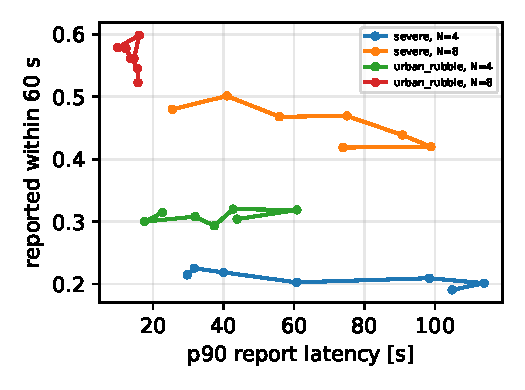
\includegraphics[width=\columnwidth]{figures/e10_thold_tradeoff.pdf}
\caption{Hold time $T_h\in\{\nThList\}$\,s: share reported within 60\,s vs.\
90th-percentile latency (mean of \nSeeds{} seeds per point).}\label{fig:thold}
\end{figure}

\emph{Link preservation.}\label{sec:safety} Over all experiments, tethered and mutually preserved links
that were reliable before a step failed after it \nViolAll{} times in \nStepsAll{} link-steps
($\nViolRate$). On the same seeds without the projection, violations rose from \nViolOn{} in \nStepsOn{}
link-steps (\nRunsOn{} run) to \nViolOff{} in \nStepsOff{} (\nRunsOff{} runs), a \nViolFold-fold
difference (paired Wilcoxon, $p<\nViolP$). Tethers are short, so this protection does not change the
on-time share measurably.

\emph{PX4/Gazebo and the earlier scenario.}\label{sec:sitl} \nEightN{} PX4 x500 UAVs flew SENTINEL and B0 in
Gazebo on \nEightWorlds{} generated \nEightArea\,m areas with one crash; reported victims, packet delivery ratio and connected time
agree with the fast simulator within \nEightMaxDiff{} (SENTINEL \nEightSitlS{} vs.\ \nEightFastS,
B0 \nEightSitlB{} vs.\ \nEightFastB). With \nEightWorlds{} seeds this is a consistency check, and in an area this
size B0 is slightly ahead in both environments. Re-running the \nNineArea\,m, \nNineN-UAV scenario of our first
version, every method stays connected throughout. That scenario has no responder, so we compare confirmed victims: SENTINEL confirms
\nNineS{} of them, B0 \nNineBzero{} (not significantly fewer) and the first version \nNineBone{}
(significantly fewer); victims closer than the \nGate\,m
association gate merge in \nNineAssocLo--\nNineAssocHi\,\% of confirmations. The network-retention
gains reported for that scenario are not reproduced, and we withdraw them.

\emph{Detector.} Trained under one protocol on HIT-UAV \cite{hituav}, YOLO26n \cite{yolo26} matches
YOLOv8n in validation mAP50 (\nYnMap{} vs.\ \nVeMap; mAP50-95 \nYnMapB{} vs.\ \nVeMapB) with
\nYnParamRed\,\% fewer parameters and \nYnFlopRed\,\% fewer operations. End-to-end TensorRT FP16
latency on a desktop RTX~3060 is \nYnTrt\,ms vs.\ \nVeTrt\,ms; embedded latency was not measured.

\section{Limitations and Conclusion}
All results come from simulation, a fast multi-agent simulator and PX4 software-in-the-loop; no
hardware flights were made. The channel is parameterised from published ranges and not calibrated in
rubble. Detection accuracy is the training run's validation result on HIT-UAV, whose imagery is taken
from higher altitudes than our \nAlt\,m; the detector transfers poorly to rendered scenes, so the loop uses
a parameterised detector model whose parameters were set by hand and swept, not fitted. Victims closer
than the association gate can merge. MAPPO was trained with one observation and reward design. Latency
was measured on a desktop GPU only.

SENTINEL treats the swarm network as an elastic mesh that stretches during search and is re-formed
for delivery. Across \nMissions{} simulated missions it reported more victims within 60\,s than seven
tuned baselines in most settings and was never significantly worse than any of them. Fusion and
information-triggered delivery had significant effects, although in dense swarms the fusion rule
alone explains the advantage, and constant connectivity reduced timely reporting. Future work
will adapt $T_h$ to the observed contact rate, calibrate the channel with measurements and fly the
system on hardware.

\bibliographystyle{IEEEtran}
\bibliography{references}
\end{document}
